% =====================================================================
%  Hi-VideoSum Midterm Report
%  Compile with: XeLaTeX  (Overleaf: Menu → Compiler → XeLaTeX)
% =====================================================================
\documentclass[11pt,a4paper]{article}

% ---------- Encoding & fonts (Korean via kotex) ----------
\usepackage{fontspec}
\usepackage[hangul]{kotex}
\setmainhangulfont{Noto Serif CJK KR}
\setsanshangulfont{Noto Sans CJK KR}
\setmonohangulfont{Noto Sans Mono CJK KR}
\setmainfont{Latin Modern Roman}
\setmonofont{Latin Modern Mono}
\XeTeXlinebreaklocale "ko"
\XeTeXlinebreakskip = 0pt plus 1pt minus 0pt

% ---------- Layout ----------
\usepackage[margin=1in]{geometry}
\usepackage{setspace}
\onehalfspacing
\usepackage{parskip}
\setlength{\parindent}{1em}

% ---------- Common packages ----------
\usepackage{graphicx}
\usepackage{caption}
\usepackage{booktabs}
\usepackage{array}
\usepackage{longtable}
\usepackage{xurl}
\usepackage{ragged2e}
\usepackage{hyperref}
\usepackage{subcaption}
\usepackage{float}
\hypersetup{
  colorlinks=false,
  pdfborder={0 0 0},
  linkbordercolor={1 1 1},
  urlbordercolor={1 1 1},
  citebordercolor={1 1 1},
  pdftitle={Hi-VideoSum Midterm Report}
}

\Urlmuskip=0mu plus 1mu
\usepackage{xcolor}
\usepackage{listings}
\lstset{
  basicstyle=\ttfamily\footnotesize,
  breaklines=true,
  breakatwhitespace=true,
  columns=fullflexible,
  frame=single,
  framesep=4pt,
  xleftmargin=4pt,
  xrightmargin=4pt,
  showstringspaces=false,
  keepspaces=true,
}

% ---------- Section title tuning ----------
\usepackage{titlesec}
\titleformat*{\section}{\Large\bfseries}
\titleformat*{\subsection}{\large\bfseries}

% =====================================================================
\begin{document}
\thispagestyle{empty}

% ---------- Title Page ----------
\vspace*{4cm}
\begin{center}
  {\Huge\bfseries Hi-VideoSum}\\[14pt]
  {\LARGE 사용자 친화적 유튜브 영상 요약 및 하이라이트 서비스}\\[24pt]
  {\Large 데이터사이언스 캡스톤 프로젝트 중간 보고서}
\end{center}

\vfill

\begin{center}
\begin{tabular}{rl}
\textbf{팀명}     & Hi-Everyone \\
\textbf{팀원}     & 정연후(2021312615), 오경준(2021313008), 이용하(2021312638), 김기표 (2021311409) \\
\textbf{과목명}   & 데이터사이언스 캡스톤 프로젝트 \\
\textbf{지도교수} & 정미나 \\
\textbf{소속학과} & 인공지능융합전공 \\
\textbf{제출일} & 2026-05-14 \\
\end{tabular}
\end{center}

\vspace{2cm}

\newpage
\setcounter{page}{1}

% =====================================================================
\section*{Abstract}
\addcontentsline{toc}{section}{Abstract}

숏폼 콘텐츠 소비가 일반화된 오늘날, 시청자들은 영상의 길이에 관계없이 핵심 내용과 다른 시청자들의 반응을 함께 빠르게 파악할 수 있는 요약 서비스에 대한 수요가 커지고 있으며, 이는 단순한 내용 압축을 넘어 시청자 관점을 함께 전달하는 사용자 친화적 요약 기술의 필요성을 부각시킨다. 그러나 현재 시장의 영상 요약 솔루션은 이러한 요구를 충분히 충족하지 못하고 있다. Monica, Livewiki와 같은 웹 기반 서비스는 영상 자체의 내용만을 요약 대상으로 삼아 시청자 반응을 전혀 반영하지 못하며, Copilot이나 Gemini와 같은 범용 멀티모달 LLM은 프롬프트 의존성이 높고 시간 구간·댓글 내용에 대한 환각 현상이 빈번하여 실용적 신뢰성이 부족하다. 더 나아가 비디오 프레임을 직접 처리하는 방식은 연산 비용이 높아 실서비스 환경에서의 안정적 운용에도 한계를 보인다. 본 프로젝트 Hi-VideoSum은 이러한 격차를 해결하기 위해, 영상 프레임을 처리하지 않고 한국어 유튜브 영상의 대본(transcript)과 시청자 댓글이라는 텍스트 데이터만으로 동작하는 자원 효율적인 sLLM 기반 요약 서비스를 구축하는 것을 목표로 한다. 이를 위해 YouTube Data API와 자막 수집 도구를 활용하여 한국 유튜브 채널 약 80개에서 영상 길이 5분에서 30분 사이의 비디오를 채널당 최대 200개 수집하고, LLM 기반의 3축 평가 체계(정보성·의견성·연관성)를 통해 고품질 댓글을 선별하는 필터링 파이프라인을 설계한다. 또한 선별된 대본·댓글을 입력으로 하고 영상 요약·시청자 반응 요약·하이라이트를 출력으로 하는 고품질 요약 레이블 생성 파이프라인을 함께 설계하여, 사용자 친화적 요약 서비스 훈련을 위한 약 1만 개 규모의 데이터셋 구축을 추진한다. 이렇게 구축된 데이터셋을 기반으로 LG Exaone, Kormo, Gemma와 같이 한국어 처리 성능이 검증된 자원 효율적 sLLM을 후보군으로 선정하고, LoRA·QLoRA·Prefix Tuning·Full Fine-tuning을 비교 실험하여 성능과 비용의 균형이 가장 우수한 파인튜닝 방법론을 도출한다. 본 프로젝트는 이상의 과정을 통해 사용자가 유튜브 URL을 입력하는 것만으로 영상 요약과 시청자 반응 하이라이트를 즉시 받아볼 수 있는 실서비스를 구현함으로써, 시청자 관점이 반영된 신뢰 가능하고 효율적인 한국어 영상 요약 서비스의 새로운 가능성을 제시하는 데 의의를 갖는다.

% =====================================================================
\section{Introduction}\label{sec:intro}

숏폼 콘텐츠 소비가 일반화된 오늘날, 시청자들은 단순히 영상의 줄거리를 압축한 결과물보다는 다른 시청자들의 공감 포인트와 반응까지 함께 빠르게 파악할 수 있는 요약을 기대한다. 즉 영상 요약은 더 이상 ``내용 압축'' 수준에 머무르지 않고, 시청자가 영상을 볼지 말지를 판단하는 사회적 단서까지 제공하는 사용자 경험의 일부로 자리 잡는 방향으로 발전되어야 한다. 그러나 이러한 사용자 기대를 정면으로 겨냥하는 현 시장의 영상 요약 솔루션들은 세 가지 측면에서 그 요구를 충분히 충족하지 못하고 있다. 첫째, Monica나 Livewiki와 같은 웹 기반 서비스는 영상 자체의 내용만을 요약 대상으로 삼아 시청자가 어떤 부분에 공감하고 반응했는지를 전혀 반영하지 못한다. 둘째, 크롬이나 유튜브의 확장 프로그램으로 지원되는 Copilot이나 Gemini와 같은 범용 멀티모달 LLM은 프롬프트 설계에 지나치게 의존하며, 특정 시간 구간이나 댓글 내용에 대해 사실과 다른 내용을 생성하는 환각(Hallucination) 현상이 빈번하게 발생하여 결과물의 신뢰성을 저해한다. 셋째, 비디오 프레임을 직접 처리하는 방식은 연산 비용이 높아 실서비스 환경에서의 안정적 운용을 어렵게 한다. 결과적으로 시청자 관점의 결여, 환각으로 인한 신뢰성 저하, 그리고 운영 비효율이라는 세 가지 격차가 동시에 해결되어야 사용자 친화적 영상 요약 서비스가 가능해진다.

본 프로젝트는 이러한 문제의식에서 출발하여, 영상 프레임을 처리하지 않고 대본과 댓글이라는 텍스트 데이터만으로 동작하는 sLLM 파인튜닝 모델을 구축함으로써 앞서 정리한 세 가지 한계를 동시에 해결하고자 한다. 본 보고서가 다루는 연구 질문은 크게 네 갈래로 나뉜다. 먼저 본 프로젝트의 가장 근본적인 전제, 즉 댓글이 시각 정보의 보완 신호로 기능할 수 있는가를 검증하는 질문이다. 시청자 댓글이 시청자 반응과 집중 장면을 담아내는 신호로 충분히 활용 가능한가, 특히 일반 댓글과 타임스탬프 댓글이 각각 시청자 반응 요약과 하이라이트 추출에 적합한 정보를 담고 있는가이다.

다음으로 수집한 데이터셋 자체에 대한 분석적 질문이 이어진다. 비디오 카테고리(엔터테인먼트·뉴스·스포츠·영화·노하우·여행·과학기술)별로 대본 길이, 댓글 양, 타임스탬프 댓글 비율, 시청자 반응의 정보성·의견성·연관성 분포가 어떻게 다르며, 각 도메인의 데이터는 어떤 고유한 특성과 프로파일을 갖는가이다.

마지막으로 모델 구축의 실효성과 효율성을 검증하는 두 가지 질문으로, 대본과 댓글을 입력으로 하고 요약과 하이라이트를 출력으로 하는 데이터로 파인튜닝된 sLLM이 범용 LLM 대비 환각 감소와 시청자 관점 반영의 두 측면에서 실제로 우수한 성능을 보이는가, 그리고 LoRA, QLoRA, Full Fine-tuning 및 LoRA 어댑터 설정의 변형 중 본 태스크에서 자원과 성능의 균형이 가장 우수한 조합은 무엇인가를 다룬다. 이상의 네 가지 연구 질문을 모두 해결하는 것을 본 프로젝트의 목표로 한다.

본 연구는 한국 유튜브의 7개 카테고리·16개 세부 카테고리를 포괄하도록 큐레이션된 약 80개 채널을 대상으로 약 6{,}000개에서 10{,}000개 규모의 요약 학습 데이터셋을 구축한다. 이어지는 \S\ref{sec:data}에서는 데이터의 출처와 수집·전처리 파이프라인을 정리하고, \S\ref{sec:method}에서는 그 위에 구축한 요약 데이터셋 생성 방법론과 모델 훈련 시 적용한 자원 효율적 파인튜닝 방법론을 설계 의도와 함께 설명한다. \S\ref{sec:results}에서는 파일럿 단계의 예비 결과와 그로부터 도출된 인사이트를, \S\ref{sec:conclusion}에서는 현재 인식되는 한계와 향후 계획을 차례로 다룬다.

% =====================================================================
\section{Data Description}\label{sec:data}

\subsection{데이터 출처}

본 프로젝트의 데이터는 한국 유튜브를 출처로 하며, 영상 메타데이터와 채널별 영상 목록 추출에는 \texttt{yt-dlp}를, 자막 수집에는 \texttt{youtube-transcript-api}를, 댓글 수집에는 \texttt{youtube-comment-downloader}를 활용한다. 대규모 수집 과정에서 발생할 수 있는 IP 차단을 완화하기 위해 자막 수집 시 Webshare의 회전 레지덴셜 프록시를 선택적으로 경유하도록 구성하였다. 데이터 수집을 위한 채널 후보군은 팀이 정의한 7개 카테고리와 16개 세부 카테고리를 균형 있게 포괄하도록 사전에 큐레이션된 약 80개 채널로 구성된다. 대표적으로 슈카월드, 셜록현준, EBS Documentary, 피식대학, 빠니보틀, ITSub잇섭, T1 Faker, KBO, 넷플릭스 코리아 등이 포함되어 있어 정보성·예능성·전문성 측면에서 다양한 스펙트럼을 확보하였다.

\subsection{원시 데이터 수집 방법}

수집 정책은 데이터 품질을 일정 수준 이상으로 담보하기 위해 비교적 엄격하게 설계되었다. 영상 길이는 5분에서 30분 사이로 한정하여 너무 짧아 요약이 무의미하거나 너무 길어 자막 처리 비용이 과도해지는 양 극단을 배제하였다. 채널당 최대 수집 영상 수는 300개로 설정하고, 각 채널 내에서는 댓글 수 내림차순으로 정렬하여 수집을 진행하되, 댓글 수 정렬이 불가능한 경우에는 조회수 내림차순을 사용한다. 일반 댓글과 타임스탬프 댓글이 각각 최소 5개 이상 확보된 영상만 학습 후보로 채택되며, 이 조건을 만족하지 못하거나 자막이 비활성화된 영상은 수집 단계에서 즉시 스킵된다. 대댓글은 토픽 일관성이 떨어지고 노이즈가 크기 때문에 일괄적으로 제외하며, 영상별 수집 상태는 \texttt{collected}, \texttt{skipped}, \texttt{error}의 세 상태로 로그에 기록되어 이후 분석에 활용된다.

수집되는 데이터의 유형은 세 가지로 구분된다. 첫째는 대본(Transcript)으로, 영상의 자동 또는 수동 자막 시퀀스이며 각 발화 구간의 시작 시각과 지속 시간 정보가 함께 저장된다. 둘째는 일반 댓글(General Comment)로, 타임스탬프가 포함되지 않은 텍스트 댓글이며 시청자들의 영상에 대한 일반적인 반응을 담을 것으로 기대되어 수집된다. 셋째는 타임스탬프 댓글(Timestamp Comment)로, \texttt{MM:SS} 또는 \texttt{HH:MM:SS} 형식의 시간 정보가 본문에 포함된 댓글이며 이는 특정 구간에 집중된 시청자의 반응을 담을 것으로 기대된다. 추출된 시간 리스트가 \texttt{timestamps\_found} 필드로 함께 저장되어 하이라이트 생성을 위한 핵심 신호로 활용된다. 영상 단위의 모든 데이터는 한 줄에 한 영상을 담는 JSONL 형식(\texttt{combined\_data.jsonl})으로 통합되며, 각 레코드는 영상 ID·제목·채널 정보·영상 길이·대본 시퀀스·일반 댓글·타임스탬프 댓글을 포함한다.

수집 시점에는 댓글 단위에도 가벼운 규칙 기반 필터링이 함께 적용되어 노이즈 댓글의 유입을 사전에 차단한다. 먼저 정규식을 이용해 댓글 본문에서 \texttt{M:SS}, \texttt{MM:SS}, \texttt{H:MM:SS} 형식의 시간 패턴을 탐지하여, 시간 정보가 포함된 댓글은 타임스탬프 댓글로, 그렇지 않은 댓글은 일반 댓글로 자동 분류한다. 일반 댓글에는 의미성(meaningfulness) 검사가 추가로 적용되는데, 공백을 제거한 본문 길이가 10자 미만이거나 한글·영문·숫자 같은 의미 문자가 10자 미만인 댓글, 그리고 전체 문자 중 의미 문자의 비율이 40\% 미만인 댓글(이모지·특수문자 도배에 해당)은 모두 제외한다. 타임스탬프 댓글은 시간 신호 자체가 중요한 학습 단서이므로 짧은 길이라도 포함시켜 정보 손실을 줄이는 한편, 영상당 일반 댓글과 타임스탬프 댓글에 대해 각각 상한을 두어 한 영상이 데이터셋 전체 분포를 지나치게 좌우하지 않도록 하였다. 또한 지역 제한(\texttt{geo\_blocked})으로 댓글·메타데이터에 접근할 수 없는 영상은 즉시 스킵 처리되어 후속 단계로 전달되지 않는다.

이상의 절차를 통해 확보된 원시 데이터에 대해서는 이후 LLM 기반의 댓글 필터링과 산문 요약 레이블 생성을 차례로 수행하여 최종 학습 데이터셋을 구축하였으며, 각 단계의 구체적인 방법론과 사용 모델·프롬프트 설계는 \S\ref{sec:method}에서 자세히 다룬다.

\subsection{원시 데이터 통계}

% 추후 작성 예정: 원시 데이터와 2차 필터링 데이터의 분포 비교, 최종 산문 요약 데이터셋 통계.

본 프로젝트에서 수집된 데이터셋은 총 9,984개의 영상 데이터로 구성되며, 카테고리별 세부 지표는 표 \ref{tab:category_stats}와 같다. 전체 데이터의 분포를 살펴보면, 영상 길이 측면에서는 600초(10분)에서 900초(15분) 사이의 영상이 가장 높은 밀집도를 보이며 중단편 콘텐츠 위주의 안정적인 분포를 형성하고 있다.

사용자 반응의 핵심인 댓글 분포의 경우, 일반 댓글은 수집 상한선인 100개에 근접한 영상이 대다수를 차지하여 풍부한 텍스트 데이터를 확보하였음을 보여준다. 반면, 타임스탬프 댓글은 영상당 5개에서 20개 사이의 적은 구간에 데이터가 집중된 롱테일(Long-tail) 분포를 띄고 있으나, 100개 이상의 타임스탬프가 밀집된 고품질 샘플 또한 상당수 존재하여 하이라이트 추출 학습을 위한 변별력을 갖추었다.

카테고리별 분포는 '엔터테인먼트'가 4,303개(43.1\%)로 가장 높고, 이어 '뉴스/시사'(1,384개), '여행/이벤트'(1,359개) 순이며, '영화/애니메이션'(540개)이 가장 적은 비중을 차지한다. 전체 영상의 평균 길이는 926.8초이며, 카테고리별로는 '여행/이벤트'가 1,019.0초로 가장 길고 '노하우/스타일'이 819.3초로 가장 짧다.

댓글 데이터의 경우 '일반 댓글'은 영상당 평균 96.6개가 수집되었으며, 카테고리 간 편차 없이 고르게 분포한다. 핵심 분석 신호인 '타임스탬프 댓글'은 전체 평균 34.0개이나 카테고리별 편차가 뚜렷하다. 특히 '여행/이벤트'는 평균 59.2개로 전체 평균의 약 1.7배를 기록하며 가장 활발한 양상을 보인 반면, '노하우/스타일'은 19.2개로 가장 낮은 분포를 기록하였다. 추가적인 데이터 분포는 부록의 그림~\ref{fig:raw_dataset_stats}에 수록되어 있다.


\begin{table}[htbp]
  \centering
  \caption{카테고리별 상세 데이터 통계}
  \vspace{3mm}
  \begin{tabular}{lrrrr}
    \toprule
    \textbf{카테고리} & \textbf{영상 데이터 수} & \textbf{평균 길이(초)} & \textbf{일반 댓글 수} & \textbf{타임스탬프 댓글 수} \\
    \midrule
    엔터테인먼트 & 4,303 & 928.6 & 97.0 & 38.0 \\
    노하우/스타일 & 873 & 819.3 & 86.6 & 19.2 \\
    영화/애니메이션 & 540 & 943.3 & 96.5 & 22.2 \\
    뉴스/시사 & 1,384 & 929.6 & 98.8 & 22.3 \\
    과학기술 & 821 & 822.8 & 97.5 & 27.1 \\
    스포츠 & 704 & 974.4 & 95.8 & 29.5 \\
    여행/이벤트 & 1,359 & 1,019.0 & 99.4 & 59.2 \\
    \midrule
    \textbf{전체 (Total)} & \textbf{9,984} & \textbf{926.8} & \textbf{96.6} & \textbf{34.0} \\
    \bottomrule
  \end{tabular}
  \label{tab:category_stats}
\end{table}

\begin{figure}[htbp]
     \centering
     % 첫 번째 행: 전체 영상 길이 및 타임스탬프 분포
     \begin{subfigure}[b]{0.48\textwidth}
         \centering
         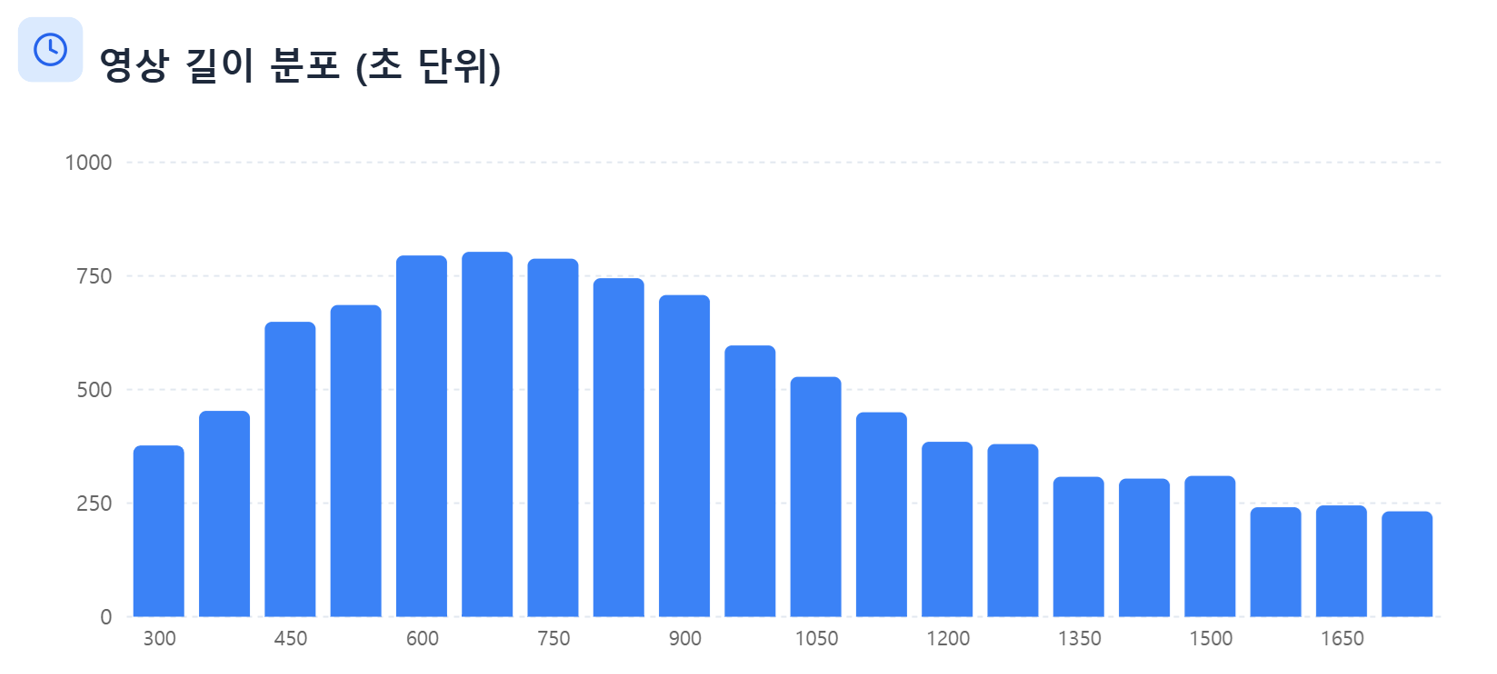
\includegraphics[width=\textwidth]{figures/raw_data_video_length.png}
         \caption{전체 영상 길이 분포}
         \label{fig:overall_len_sep}
     \end{subfigure}
     \hfill
     \begin{subfigure}[b]{0.48\textwidth}
         \centering
         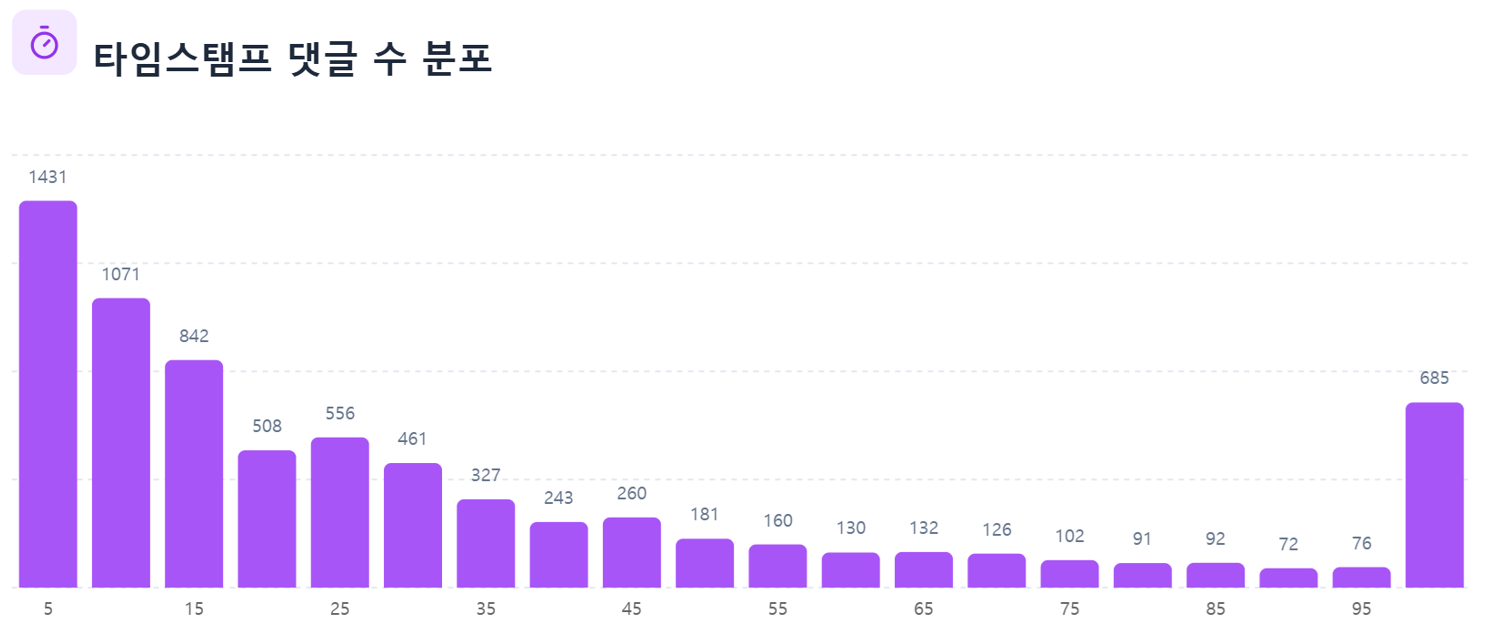
\includegraphics[width=\textwidth]{figures/raw_data_timestamp_comment.png}
         \caption{전체 타임스탬프 분포}
         \label{fig:overall_time_sep}
     \end{subfigure}
     
     \caption{데이터셋 시간 지표 분포(영상 길이 및 타임스탬프)}
     \label{fig:dataset_time_stats}
\end{figure}

\subsection{데이터 전처리}
수집된 원시 데이터의 정제 및 가공을 위한 구체적인 전처리 과정은 \S\ref{sec:method}에서 상세히 다룬다. 해당 절에서 설명하는 LLM 기반 댓글 필터링 파이프라인 및 요약 데이터 생성 방법론을 통해, 수집된 텍스트 데이터가 최종 학습용 데이터셋으로 변환되는 과정을 확인할 수 있다.

\subsection{윤리·법적 측면}
본 프로젝트는 데이터 수집·활용 전반에 걸쳐 다음 사항을 준수한다. 댓글 작성자의 ID나 프로필 식별자는 수집 단계에서 제외하고 본문만을 저장하여 개인정보 보호를 확보하며, 영상 원본은 저장하지 않고 자막과 댓글의 텍스트만 활용함으로써 저작권 이슈를 회피한다. 본 데이터는 학술 연구 목적에 한정하여 활용되며, 유튜브 약관이 허용하는 범위 내에서만 수집된다. 또한 폭력적이거나 혐오를 조장하는 표현은 후속 LLM 필터 단계에서 추가로 제거하여 모델 학습에 미치는 부정적 영향을 최소화한다.

% =====================================================================
\section{Methodology}\label{sec:method}

\begin{figure}[h]
  \centering
  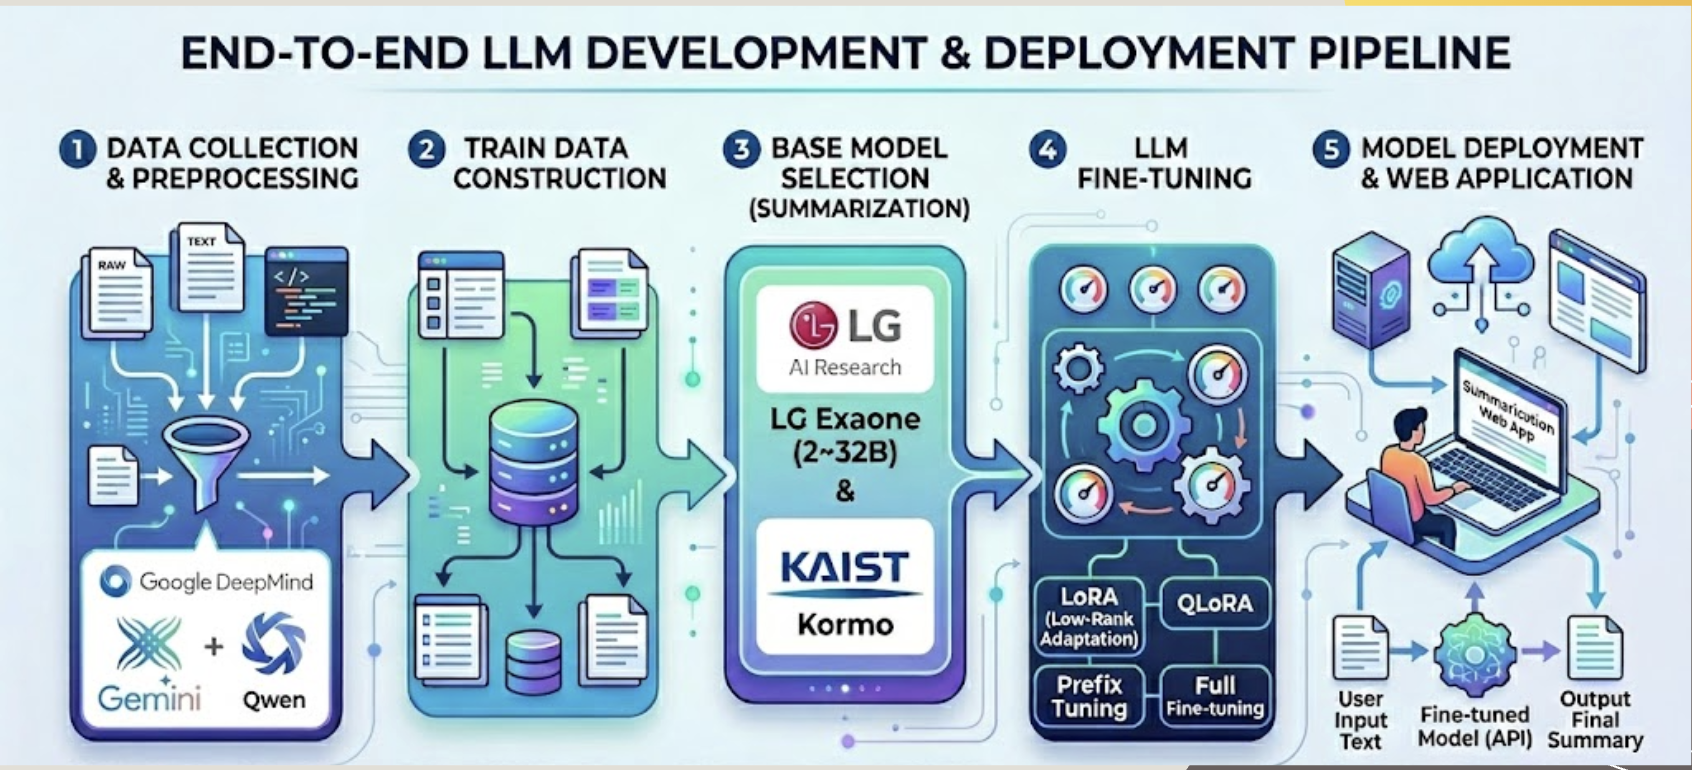
\includegraphics[width=0.95\linewidth]{figures/pipeline.png}
  \caption{Hi-VideoSum 전체 파이프라인 개요. 채널 큐레이션·원시 데이터 수집(\S\ref{sec:data})을 시작으로, LLM 기반 댓글 필터링, 산문 요약 레이블 생성, sLLM LoRA 파인튜닝을 거쳐 최종 웹 서비스로 배포되는 6단계 흐름을 나타낸다.}
  \label{fig:pipeline}
\end{figure}

본 프로젝트의 전체 파이프라인은 데이터 수집부터 모델 배포까지 여섯 단계로 구성되며, 그 전체 구조는 그림~\ref{fig:pipeline}에 도식화되어 있다. 먼저 큐레이션된 채널 리스트에서 출발하여 영상·대본·댓글(일반 댓글, 타임스탬프 댓글)을 수집하고, 수집 시점의 규칙 기반 필터링과 LLM을 활용한 3축(정보성·의견성·연관성) 평가 기반 댓글 필터링을 차례로 거친다. 이어 정제된 데이터로 산문 형식의 요약 레이블을 생성하여 학습 페어를 구축한 뒤, 이를 활용해 sLLM을 여러 LoRA 방식으로 파인튜닝하고, 마지막으로 평가를 통과한 모델을 웹 서비스로 배포한다. 여섯 단계 중 채널 큐레이션과 원시 데이터 수집은 \S\ref{sec:data}에서 이미 다루었으므로, 본 절에서는 그 위에 적용되는 LLM 기반 정제 절차부터 모델 학습에 이르는 후속 단계를 본격적으로 설명한다.

\subsection{댓글 2차 필터링}
방법론의 핵심을 이루는 댓글 필터링은 \S\ref{sec:data}에서 정리한 수집 시점의 규칙 기반 1차 필터링 위에 적용되는 2차 정제 단계로, LLM에 정형화된 평가 프롬프트를 제공하여 수행된다. 평가는 세 가지 축으로 나뉘는데, 정보성은 댓글 자체가 담고 있는 정보의 풍부함을 1점에서 3점으로 평가하고, 의견성은 시청자의 주관적 의견과 감정의 표현 정도를 같은 척도로 평가하며, 연관성은 댓글이 대본의 구체적 내용 즉 영상의 내용과 얼마나 직접적으로 연결되는지를 평가한다. 각 댓글에는 총점 3점에서 9점 사이의 점수가 부여되며, 본 프로젝트에서는 파일럿 결과를 바탕으로 \textbf{총점 6점 이상}인 댓글만을 최종 학습 후보로 채택하기로 결정하였다. 이 과정에서 댓글별 정보성·의견성·연관성 세부 점수와 총점, Pass/Fail 판정 결과가 함께 저장된다. 필터링 모델로는 K-EXAONE 238B(Elice API)를 단독으로 활용하여 모든 영상의 댓글에 동일 프롬프트를 적용하였으며, 실제 사용된 3축 평가 프롬프트의 전문은 부록의 그림~\ref{fig:filterprompt_image}에 수록되어 있다.

\subsection{요약 데이터}
최종적인 모델 학습을 위한 요약 데이터는 정제된 댓글과 전체 대본을 입력으로 받아, 영상 내용·시청자 반응·집중 장면의 세 측면을 한 편의 자연스러운 산문으로 통합하는 방식으로 생성된다. 이는 본 프로젝트가 지향하는 ``사용자 친화적 요약''의 핵심 설계로, 섹션 제목이나 불릿 포인트로 정보를 나열하는 대신 500자에서 1{,}000자 내외의 친근한 `-요/-이에요' 체 문장으로 시청자에게 전달한다. 산문은 세 문단으로 구성되며, 1문단에서는 자막만을 근거로 영상의 전체 흐름을 서술하고, 2문단에서는 일반 댓글만을 근거로 시청자들의 전반적인 반응과 여론을 정리하며, 3문단에서는 타임스탬프 댓글에 기록된 시각 정보(예: ``3:24에서는'', ``7:10 부근에서는'')를 자연스럽게 녹여 시청자들이 특히 집중한 장면을 묘사한다. 각 문단의 출처를 엄격히 분리하고 자막·댓글에 없는 내용은 일절 생성하지 않도록 시스템 프롬프트 수준에서 제약함으로써 환각을 구조적으로 억제하였다. 레이블러 후보로는 Gemini 3.1 Flash Preview, EXAONE 4.0$\cdot$4.5, K-EXAONE을 모두 vLLM 및 API 호출 코드로 준비하였으며, 본 보고서 작성 시점에서는 출력 품질과 비용·속도의 균형을 고려하여 \textbf{Gemini 3.1 Flash Preview를 1차 레이블러로 단독 채택}하였다. 실제 사용된 산문 요약 프롬프트의 전문 역시 부록의 그림~\ref{fig:summaryprompt_image}에 수록되어 있다.

\subsection{모델 훈련}
본 보고서 작성 시점에서는 위 후보군 중 비교적 가벼운 \texttt{google/gemma-4-E4B-it}를 1차 베이스라인으로 채택하여 학습을 진행하고 있다. 이는 모델 크기를 비교적 작게 가져가 학습 파이프라인이 데이터·하이퍼파라미터·평가 절차 전반에 걸쳐 정상적으로 동작하는지를 빠르게 검증하고, 후속 비교 실험의 기준선을 먼저 확보하기 위한 의도된 선택이다. 향후에는 EXAONE 4.5와 Qwen 3.6 등 더 큰 규모의 한국어 sLLM에 대해서도 동일한 학습 파이프라인을 적용하여 모델 크기·아키텍처에 따른 요약 품질과 자원 효율성의 trade-off를 본격적으로 비교 실험할 계획이다.

파인튜닝은 자원 효율성을 최우선으로 두어 \textbf{LoRA 기반 방식}으로 진행한다. 당초 LoRA, QLoRA, Full Fine-tuning의 3가지 방법을 비교 실험하는 것을 계획한다. 다만 동일한 LoRA 방식 내에서도 rank, alpha, target module 구성 등을 달리한 여러 변형을 비교하여 본 태스크에 최적인 어댑터 설정을 도출할 예정이다. 현재 베이스라인 학습에서는 rank 32, alpha 64, dropout 0.05를 적용하고 있으며, 어댑터는 모델의 언어 모델 부분에 한정하여 query, key, value, output projection layer를 LoRA adapter 적용 대상으로 선정하였다. 멀티모달 입력을 지원하는 Gemma 4의 비전·오디오 인코더 타워는 동결하여 학습 대상에서 제외함으로써, 전체 파라미터 중 약 0.1$\sim$0.3\%만이 실제 학습 대상이 된다.

학습 환경은 단일 H200 GPU에서 bf16 전체 정밀도로 학습을 수행하며, 최대 시퀀스 길이를 20{,}000 토큰으로 설정하여 긴 대본·댓글 입력을 자르지 않고 한 번에 처리할 수 있도록 하였다. 옵티마이저는 AdamW 계열을 사용하고, 학습률은 $2\!\times\!10^{-4}$에서 시작하여 cosine 스케줄로 감쇠시키며 초기 3\%의 warmup을 둔다. 디바이스당 배치 크기는 8, gradient accumulation은 2로 설정하여 유효 배치 크기 16을 확보하고, gradient checkpointing을 활성화하여 활성화 재계산으로 VRAM을 추가 절약한다. 학습은 SFTTrainer를 활용해 3 에폭 동안 진행되며, 모든 학습 지표는 Weights \& Biases로 자동 기록하여 모니터링한다. 후속의 더 큰 모델 실험에서도 동일한 학습 환경과 LoRA 설정 변형 전략을 일관되게 적용하여 모델 간 비교의 공정성을 확보할 계획이다.

데이터 분할은 학습-검증-테스트 비율을 8:1:1로 두되, 같은 채널의 영상이 여러 분할에 분산되지 않도록 하여 학습 중 out-of-domain(OOD) 채널에서의 일반화 성능을 모니터링 및 최종 평가에서 확인하기 위해 채널 단위로 분할하는 channel-disjoint split을 수행한다. 검증 및 테스트에서의 평가는 자동 지표와 정성 평가를 병행하며, 자동 지표로는 ROUGE-L, 한국어 임베딩 기반 BERTScore를 활용하고, 환각 측면에서는 타임스탬프 일치율과 댓글 근거 정합률을 LLM-as-a-Judge 방식으로 측정한다. 정성 평가는 가독성, 시청자 반응 반영, 사실성의 세 항목을 5점 척도로 측정하는 방식으로 진행한다. 구축된 학습 데이터셋은 재현성과 후속 연구를 위해 HuggingFace Hub \href{https://huggingface.co/datasets/kim586w/hivideosum_training_dataset}{\texttt{kim586w/hivideosum\_training\_dataset}} 저장소에 공개되어 있다.

% =====================================================================
\section{Results and Discussion}\label{sec:results}

본 보고서 작성 시점에서는 데이터 수집과 LLM 기반 정제, 산문 요약 레이블 생성 파이프라인의 구축이 마무리 단계에 있으며, 베이스라인 모델인 \texttt{google/gemma-4-E4B-it}에 대한 LoRA 파인튜닝이 진행 중이다. 따라서 본 절에서는 현재 시점에서 보고할 수 있는 정량적 결과를 제시하기보다는, 본 프로젝트가 산출할 예비 결과의 형태와 그것을 \S\ref{sec:intro}의 연구 질문과 어떻게 연결지어 해석할 것인지, 그리고 분석 과정에서 예상되는 인사이트와 한계점을 정리한다.

\subsection{데이터 정제 및 필터링 결과 분석}\label{subsec:filter_res}

본 연구에서는 고품질의 요약 및 하이라이트 레이블 생성을 위해 LLM(K-EXAONE 238B) 기반의 3축 평가 필터링을 수행하였다. 필터링 결과, 전체 1,290,795개의 댓글 중 약 63.15\%인 815,177개의 댓글이 최종 학습 데이터셋으로 선별되었다.

댓글 유형별 통과율을 분석한 결과, 일반 댓글은 64.82\%의 통과율을 보였으나, 타임스탬프 댓글은 58.33\%로 상대적으로 낮게 나타났다. 이는 타임스탬프 댓글이 정보성 지표에서 평균 1.63점으로 일반 댓글(1.80점)보다 낮게 평가된 점에 기인한다. 그러나 타임스탬프 댓글의 연관성(Relevance) 점수는 2.24점으로 일반 댓글(2.24점)과 대등하게 높게 나타나, 특정 장면과 직결된 양질의 하이라이트 신호를 확보했음을 입증한다. 전체 3축 평가의 상세 통계는 표 \ref{tab:filter_results}와 같다.

\begin{table}[htbp]
  \centering
  \caption{LLM 기반 댓글 2차 필터링 및 3축 평가 통계 요약}
  \vspace{3mm}
  \begin{tabular}{lcccc}
    \toprule
    \textbf{구분} & \textbf{전체 댓글} & \textbf{일반 댓글} & \textbf{타임스탬프 댓글} \\
    \midrule
    총 수집 개수 & 1,290,795 & 959,863 & 330,932 \\
    최종 통과 개수 (Pass) & 815,177 & 622,137 & 193,040 \\
    \textbf{최종 통과율 (\%)} & \textbf{63.15\%} & \textbf{64.82\%} & \textbf{58.33\%} \\
    \midrule
    \multicolumn{4}{l}{\textit{3축 평가 평균 점수 (1.0 $\sim$ 3.0)}} \\
    \hspace{1em} 정보성 (Information) & 1.76 & 1.80 & 1.63 \\
    \hspace{1em} 의견성 (Opinion) & 2.18 & 2.20 & 2.12 \\
    \hspace{1em} 연관성 (Relevance) & 2.24 & 2.24 & 2.24 \\
    \midrule
    \textbf{총점 평균 (Total Score)} & \textbf{6.17} & \textbf{6.23} & \textbf{6.00} \\
    \bottomrule
  \end{tabular}
  \label{tab:filter_results}
\end{table}

\subsection{카테고리별 도메인 특성과 프로파일}\label{subsec:domain_analysis}

본 연구에서 정의한 7개 카테고리에 따라 대본 및 댓글 데이터의 특성을 분석한 결과, 각 도메인이 고유한 데이터 프로파일을 형성하고 있음을 확인하였다.

첫째, \textbf{대본 길이와 정보 밀도} 측면에서 과학기술(7,474.7자), 뉴스(7,350.9자), 스포츠(6,877.7자) 카테고리가 높은 평균 길이를 기록하였다. 특히 뉴스는 정보성 점수가 1.86점으로 전체 카테고리 중 가장 높아, 텍스트 중심의 사실적 정보 요약에 적합한 도메인임을 확인하였다. 반면 여행(4,581.4자)과 영화(6,405.4자) 카테고리는 상대적으로 짧은 대본 구성을 보였다.

둘째, \textbf{시청자 참여 양상}을 나타내는 타임스탬프 댓글 비율은 여행(30.13\%)과 엔터테인먼트(29.67\%)에서 압도적으로 높게 나타났다. 이는 해당 도메인이 특정 시간대 장면을 중심으로 시청자 반응이 집중되는 특성을 갖는다는 것을 보여준다.

셋째, \textbf{반응의 성격} 분석 결과 노하우/스타일(2.33점) 카테고리의 의견성 점수가 가장 높게 측정되었으며, 스포츠(2.24점)와 여행(2.23점)이 그 뒤를 잇는다. 이는 단순한 내용 요약을 넘어 시청자들의 감정적 호응과 공감 포인트를 반영하는 사용자 친화적 요약의 필요성을 뒷받침한다. 이러한 도메인별 특성을 반영한 핵심 지표 요약은 표 \ref{tab:domain_summary}와 같다.

종합하면 카테고리별로 대비되는 프로파일이 관찰된다. 뉴스/시사는 긴 대본과 높은 정보성을 갖춘 정보 중심 도메인으로 자막 기반 요약 비중이 크며, 엔터테인먼트와 여행/이벤트는 비교적 짧은 대본 위에 타임스탬프 댓글 비율이 30\% 내외로 높아 특정 장면에 대한 반응이 풍부하게 축적된 도메인이다. 노하우/스타일과 스포츠는 의견성·연관성 점수가 동시에 높아 시청자의 주관적 평가와 공감이 두드러지는 도메인으로 분류된다. 한편 과학기술은 대본 길이가 가장 길지만 정보성 점수는 상대적으로 낮아, 긴 설명형 대본 위에 정보성보다는 호기심·감탄성 댓글이 주를 이루는 고유한 프로파일을 보인다.

\begin{table}[htbp]
  \centering
  \caption{카테고리별 주요 도메인 지표 요약}
  \vspace{3mm}
  \begin{tabular}{lccccc}
    \toprule
    \textbf{카테고리} & \textbf{평균 대본 길이} & \textbf{타임스탬프 비율} & \textbf{정보성 평균} & \textbf{의견성 평균} & \textbf{연관성 평균} \\
    \midrule
    과학기술 & \textbf{7,474.7} & 21.77\% & 1.70 & 2.03 & 2.08 \\
    뉴스/시사 & 7,350.9 & 17.10\% & 1.86 & 2.08 & 2.16 \\
    스포츠 & 6,877.7 & 23.66\% & 1.76 & 2.24 & 2.31 \\
    영화/애니메이션 & 6,405.4 & 16.25\% & 1.72 & 2.06 & 2.14 \\
    노하우/스타일 & 5,516.7 & 18.48\% & 1.76 & 2.33 & 2.41 \\
    엔터테인먼트 & 5,587.9 & 29.67\% & 1.73 & 2.20 & 2.25 \\
    여행/이벤트 & 4,581.4 & \textbf{30.13}\% & 1.78 & 2.23 & 2.27 \\
    \bottomrule
  \end{tabular}
  \label{tab:domain_summary}
\end{table}

\subsection{예비 결과의 제시 계획}\label{subsec:prelim}

예비 결과는 크게 세 층위로 정리될 예정이다. 첫째, \textbf{데이터셋 수준의 통계}로서 \S\ref{sec:data}에서 다룰 원시 데이터와 LLM 필터링을 거친 2차 데이터의 분포 비교, 그리고 최종 산문 요약 데이터셋의 길이·문단 구성 분포를 표와 히스토그램 형태로 제시한다. 둘째, \textbf{필터링 단계의 산출물}로서 K-EXAONE 238B 기반 3축 점수의 카테고리별·축별 분포를 시각화하고, 임계값 6점 채택 전후의 Pass 비율 변화와 통과 댓글의 정성적 특징을 사례 중심으로 제시한다. 셋째, \textbf{모델 학습 결과}로서 베이스라인 Gemma 4 E4B-it의 학습 곡선(W\&B 로깅 기반 train/validation loss, ROUGE-L, BERTScore)과 후속으로 진행될 EXAONE 4.5$\cdot$Qwen 3.6 등 더 큰 모델과의 성능·자원 효율성 비교 표를 함께 제시할 예정이다.

\subsection{결과 해석과 연구 질문의 연관성}

도출된 결과는 \S\ref{sec:intro}에서 제시한 네 가지 연구 질문과 직접적으로 연결된다. 먼저 \textbf{RQ1(댓글의 보완 신호로서의 충분성)}에 대해서는, \S\ref{subsec:filter_res}의 3축 필터링 결과가 직접적인 답을 제공한다. 일반 댓글은 통과율(64.82\%)과 정보성 점수(1.80)가 상대적으로 높아 시청자 반응 요약에 안정적으로 활용될 수 있으며, 타임스탬프 댓글은 정보성은 낮지만 연관성 점수(2.24)가 일반 댓글과 동등하게 높아 특정 시간대의 집중 장면을 찾는 데 유용하다는 점이 확인된다. 이는 본 프로젝트의 3문단 산문 요약 구조 중 2문단(일반 댓글 기반 시청자 반응)과 3문단(타임스탬프 댓글 기반 집중 장면)을 댓글 데이터만으로도 안정적으로 채울 수 있음을 뒷받침한다.

\textbf{RQ2(도메인별 데이터 특성과 프로파일)}에 대해서는 \S\ref{subsec:domain_analysis}의 카테고리별 분석이 직접적인 답이 된다. 카테고리별로 대본 길이, 타임스탬프 비율, 3축 점수가 뚜렷하게 차이를 보이며, 뉴스/시사는 정보 중심 도메인, 엔터테인먼트·여행/이벤트는 장면 반응형 도메인, 노하우/스타일·스포츠는 시청자 공감형 도메인, 과학기술은 긴 대본 위에 호기심·감탄성 댓글이 주를 이루는 고유한 프로파일로 정리된다.

\textbf{RQ3(파인튜닝 sLLM 대 범용 LLM)}과 \textbf{RQ4(LoRA 설정·모델 조합의 자원-성능 균형)}에 대해서는 \S\ref{subsec:prelim}에 정리한 베이스라인 학습 곡선·자동 지표·환각 측정 결과와, 후속으로 진행될 EXAONE 4.5·Qwen 3.6 등 더 큰 모델 및 LoRA 어댑터 설정 변형 간 비교 실험 결과가 정량적 근거를 제시할 것이다.

\subsection{예상되는 주요 인사이트와 관찰 패턴}

본 프로젝트의 설계상 다음과 같은 패턴이 관찰될 것으로 예상한다. 우선 시청자 반응을 함께 요약한 결과물이 영상 내용만을 압축한 결과 대비 사용자의 공감·흥미 차원에서 더 높은 정성 평가를 받을 것으로 기대된다. 또한 타임스탬프 댓글이 충분히 확보된 영상에서는 산문 3문단 중 집중 장면 문단의 구체성이 두드러져, 시청자가 직접 지목한 시각 정보가 강력한 학습 신호로 작용할 것으로 보인다. 카테고리 측면에서는 뉴스·과학기술과 같이 정보 중심 구성을 가진 도메인이 엔터테인먼트·문화 도메인보다 요약 품질 안정성이 높게 나타날 가능성이 있으며, 이는 도메인별 평가 결과를 분리해 제시함으로써 검증할 예정이다.

\subsection{분석의 한계와 제약}

본 프로젝트가 도출할 결과를 해석할 때 다음의 한계가 함께 고려되어야 한다. 첫째, 유튜브 자체의 데이터 분포의 영향으로 인해 채널 큐레이션 단계에서 카테고리 간 영상 분포가 완전히 균형 잡혀 있지 않으며, 특히 엔터테인먼트 비중이 상대적으로 크다는 점이 데이터 편향으로 작용할 가능성이 있다. 둘째, 수집된 자막 중 자동 생성 자막도 포함되어 있기에 음성 인식 오류가 요약에까지 전파될 수 있다. 셋째, 학습 레이블 자체가 LLM(Gemini 3.1 Flash Preview)이 생성한 산출물이라는 점에서 레이블러의 편향이 파인튜닝 모델에 내재화될 위험이 있다.

% =====================================================================
\section{Conclusion}\label{sec:conclusion}

본 중간 보고서까지 정리된 핵심 성과는 세 가지로 요약된다. 첫째, 7개 카테고리·약 80개 채널에 대해 자막과 댓글만을 활용하는 텍스트 전용 수집 파이프라인을 구축하고, 영상 길이·댓글 개수 등의 수집 조건과 타임스탬프 자동 분류·의미성 검사 등의 규칙 기반 필터링으로 노이즈를 사전에 차단하였다. 둘째, 그 위에 LLM 기반 3축(정보성·의견성·연관성) 평가로 시청자 반응 품질이 검증된 댓글을 선별하고, 정제된 대본과 댓글로부터 영상 내용·시청자 반응·집중 장면의 3문단 산문 요약을 생성하는 레이블링 파이프라인을 완성하여 약 1만 개 규모의 학습 데이터셋 구축을 진행하고 있다. 셋째, 비교적 가벼운 한국어 sLLM을 베이스라인으로 LoRA 파인튜닝을 진행하여 단일 GPU 환경에서의 학습 파이프라인 정상 동작과 자원 효율성을 확인하였다.

최종적으로 구축될 요약 서비스는 영상 내용·시청자 반응·집중 장면을 함께 담아냄으로써, 기존 서비스가 놓치고 있던 사용자 관점을 결과물에 자연스럽게 녹여 낼 것으로 기대된다. 또한 LLM 기반 3축 평가로 노이즈 댓글을 사전 차단하고 시스템 프롬프트 수준에서 문단별 출처를 엄격히 분리하는 설계를 통해, 자막·댓글에 없는 내용이 산문에 끼어드는 환각을 구조적으로 억제하여 결과물의 신뢰성을 높일 것으로 예상된다. 더 나아가 영상 프레임을 전혀 처리하지 않고 텍스트 데이터만으로 동작하는 자원 효율적 sLLM 파인튜닝 체계를 채택함으로써, 연산·운용 비용을 크게 낮추어 실서비스 환경에서도 안정적으로 운용 가능한 서비스로 이어질 것으로 전망된다. 이로써 본 프로젝트는 단순한 내용 압축을 넘어 시청자가 영상을 선택할 때 활용하는 사회적 단서까지 전달하는 사용자 친화적 요약 서비스로의 발전 가능성을 제시하며, 사용된 코드·프롬프트와 학습 데이터셋을 공개함으로써 한국어 영상 요약 분야의 데이터·도구 공동 자산으로 기능하여 해당 분야의 서비스 발전과 연구에 기여할 것으로 기대된다.

향후에는 현재 훈련 진행 중인 베이스라인 모델을 출발점으로 더 큰 규모의 한국어 sLLM과 LoRA 변형 설정을 비교 실험하여 본 태스크에 가장 적합한 모델·어댑터 조합을 도출할 계획이다. 이어 자동 지표·정성 평가·환각 측정을 종합한 최종 모델 선정과 웹 서비스 배포를 진행하여, 사용자가 유튜브 URL 입력만으로 요약 결과를 즉시 받아볼 수 있는 실서비스로 프로젝트를 완성할 예정이다.

% =====================================================================
\appendix
\section*{Appendix}
\addcontentsline{toc}{section}{Appendix}

\subsection*{A. 댓글 필터링 프롬프트}
\addcontentsline{toc}{subsection}{A. 댓글 필터링 프롬프트}

\begin{figure}[H]
    \centering
    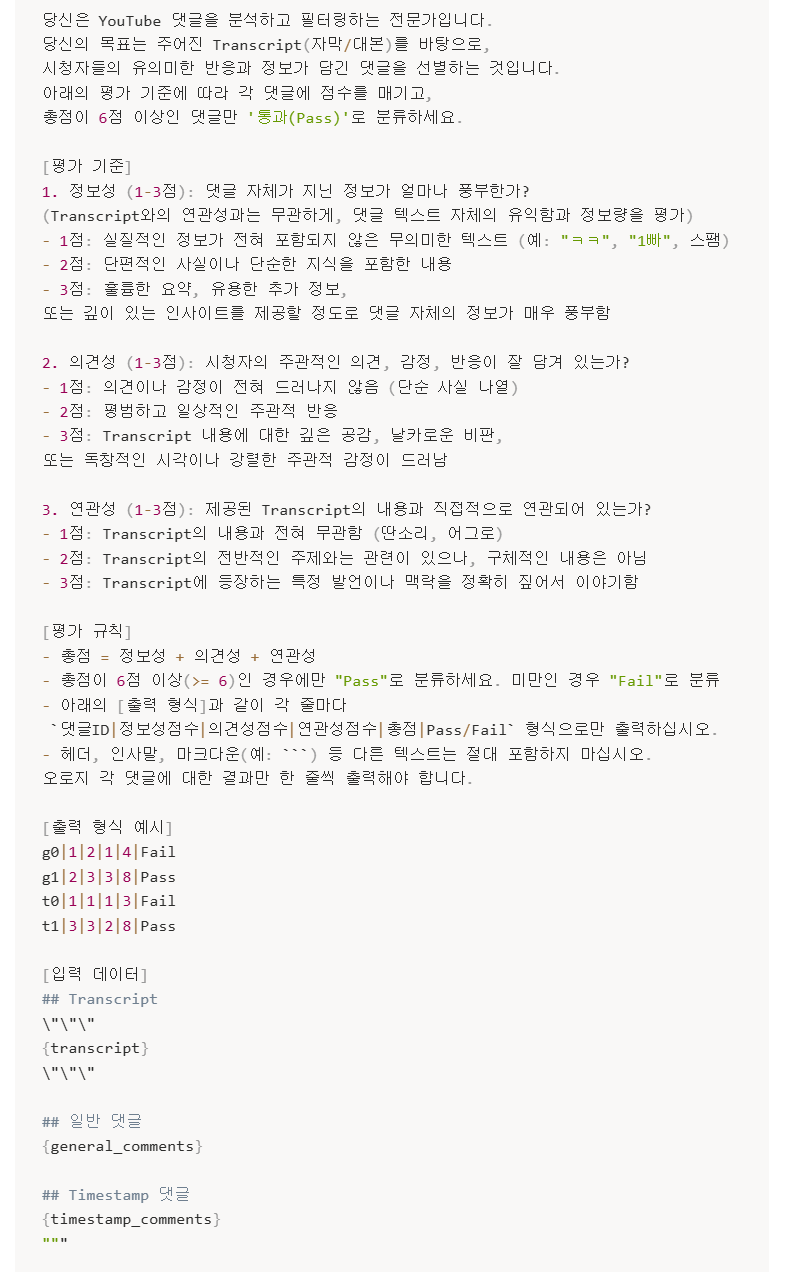
\includegraphics[width=\textwidth,height=0.9\textheight,keepaspectratio]{figures/filtering_prompt.png}
    \caption{댓글 필터링에 사용된 3축 평가 프롬프트. 정보성, 의견성, 연관성 기준에 따라 각 댓글을 평가하고, 총점 6점 이상의 댓글만 최종 학습 데이터로 채택하도록 설계하였다.}
    \label{fig:filterprompt_image}
\end{figure}
% ---------------------------------------------------------------------
\clearpage


\subsection*{B. 산문 요약 생성 프롬프트}
\addcontentsline{toc}{subsection}{B. 산문 요약 생성 프롬프트}

\begin{figure}[H]
    \centering
    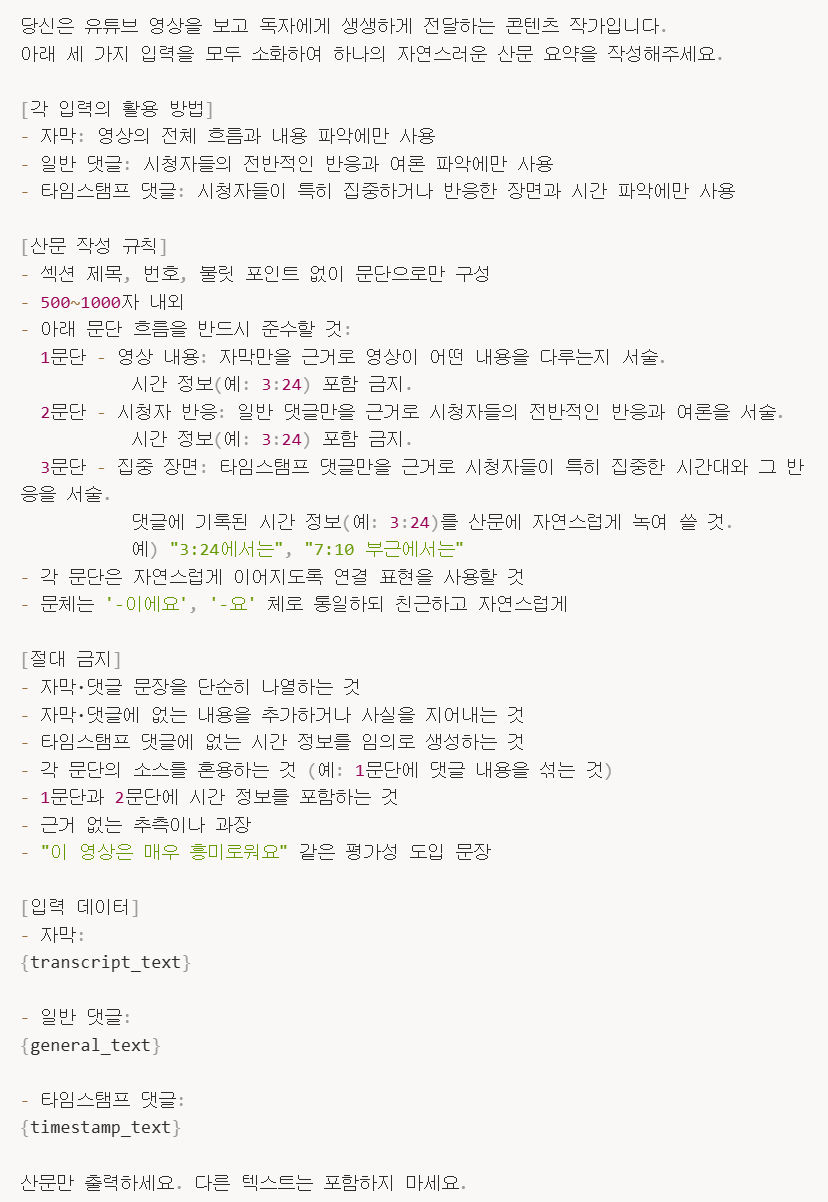
\includegraphics[width=0.95\textwidth]{figures/image.png}
    \caption{최종 요약 데이터셋 생성에 사용된 산문 요약 프롬프트. 영상 내용, 시청자 반응, 집중 장면의 3문단 구조와 출처 분리 규칙을 명시함으로써, 환각 및 출처 혼용을 구조적으로 억제한다.}
    \label{fig:summaryprompt_image}
\end{figure}

\clearpage


\subsection*{C. Channel List}
\addcontentsline{toc}{subsection}{C. Channel List}

\begingroup
\tiny
\sloppy
\emergencystretch=3em
\renewcommand{\arraystretch}{1.08}
\setlength{\tabcolsep}{2pt}
\setlength\LTleft{0pt}
\setlength\LTright{0pt}

\begin{longtable}{
@{}
>{\RaggedRight\arraybackslash}p{0.18\textwidth}
>{\RaggedRight\arraybackslash}p{0.46\textwidth}
>{\RaggedRight\arraybackslash}p{0.17\textwidth}
>{\RaggedRight\arraybackslash}p{0.17\textwidth}
@{}
}
\caption{Channel Lists}\\
\toprule
\textbf{Channel Name} & \textbf{URL} & \textbf{Category} & \textbf{Sub-Category} \\
\midrule
\endfirsthead

\toprule
\textbf{Channel Name} & \textbf{URL} & \textbf{Category} & \textbf{Sub-Category} \\
\midrule
\endhead

드리고 & \url{https://www.youtube.com/@drygogo} & 노하우/스타일 & 패션 \\
우주하마 & \url{https://www.youtube.com/@uzuhama} & 엔터테인먼트 & 게임 \\
꼰대희 & \url{https://www.youtube.com/@ggondaehee} & 엔터테인먼트 & 개그 \\
오티티 & \url{https://www.youtube.com/@오티티} & 영화/애니메이션 & 영화 요약 \\
kiu기우쌤 & \url{https://www.youtube.com/@kiudesign} & 노하우/스타일 & 패션 \\
강형욱의 보듬 TV & \url{https://www.youtube.com/@Bodeumofficial} & 노하우/스타일 & 생활 실험 \\
당신이 몰랐던 이야기 & \url{https://www.youtube.com/@dangmolee} & 뉴스/시사 & 시사 \\
머니그라피 Moneygraphy & \url{https://www.youtube.com/@Moneygraphy} & 뉴스/시사 & 시사 \\
B tv 이동진의 파이아키아 & \url{https://www.youtube.com/@Btv%EC%9D%B4%EB%8F%99%EC%A7%84%EC%9D%98%ED%8C%8C%EC%9D%B4%EC%95%84%ED%82%A4%EC%95%84} & 영화/애니메이션 & 영화 요약 \\
빠더너스 BDNS & \url{https://www.youtube.com/@bdns} & 엔터테인먼트 & 개그 \\
이대호 [RE:DAEHO] & \url{https://www.youtube.com/@DAEHO10} & 스포츠 & 스포츠 요약 \\
ootb STUDIO & \url{https://www.youtube.com/@ootbstudio} & 엔터테인먼트 & 생활 실험 \\
EBSDocumentary & \url{https://www.youtube.com/EBSDocumentary} & 뉴스/시사 & 자연 다큐 \\
카더정원 & \url{https://www.youtube.com/@carthejungwon} & 엔터테인먼트 & 개그 \\
오늘의 주우재 & \url{https://www.youtube.com/@todaysjoowoojae} & 노하우/스타일 & 패션 \\
오사카에사는사람들TV & \url{https://www.youtube.com/@osaka544} & 여행/이벤트 & 먹방 \& 맛집탐방 \\
김종국 GYM JONG KOOK & \url{https://www.youtube.com/@GYMJONGKOOK} & 스포츠 & 헬스 \\
긍정맨 & \url{https://www.youtube.com/@긍정맨입니다} & 여행/이벤트 & 여행 \\
계곡은개골개골 & \url{https://www.youtube.com/@waterfall_jang} & 여행/이벤트 & 여행 \\
또모 TOWMOO & \url{https://www.youtube.com/@TOWMOO} & 엔터테인먼트 & 문화 \\
육식맨 & \url{https://www.youtube.com/@YOOXICMAN} & 엔터테인먼트 & 먹방 \& 맛집탐방 \\
movie trip 무비트립 & \url{https://www.youtube.com/@movietrip_official} & 영화/애니메이션 & 영화 요약 \\
넷플릭스 코리아 & \url{https://www.youtube.com/@NetflixKorea/videos} & 영화/애니메이션 & 문화 \\
드림텔러 DREAM TELLER & \url{https://www.youtube.com/@dreamteller407} & 영화/애니메이션 & 영화 요약 \\
넷플릭스 뽕뽑기 [엘플릭스] & \url{https://www.youtube.com/@LPLIX} & 영화/애니메이션 & 영화 요약 \\
ITSub잇섭 & \url{https://www.youtube.com/@ITSUB} & 과학기술 & IT \\
UnderKg & \url{https://www.youtube.com/@Underkg} & 과학기술 & IT \\
빅페이스 & \url{https://www.youtube.com/@bigfacetv} & 엔터테인먼트 & 먹방 \& 맛집탐방 \\
먹보스 쭈엽이 & \url{https://www.youtube.com/@mukboss_jjooyup} & 엔터테인먼트 & 먹방 \& 맛집탐방 \\
정육왕 & \url{https://www.youtube.com/@meatcreator} & 엔터테인먼트 & 먹방 \& 맛집탐방 \\
마리아주 & \url{https://www.youtube.com/@mariage_in} & 엔터테인먼트 & 먹방 \& 맛집탐방 \\
먹갱 & \url{https://www.youtube.com/channel/UCGOYrCwp_ks0b4f6XQwaS4Q} & 엔터테인먼트 & 먹방 \& 맛집탐방 \\
별별역사 & \url{https://www.youtube.com/@%EB%B3%84%EB%B3%84%EC%97%AD%EC%82%AC} & 뉴스/시사 & 시사 \\
셜록현준 & \url{https://www.youtube.com/@Sherlock_HJ} & 뉴스/시사 & 시사 \\
너진똑 NJT BOOK & \url{https://www.youtube.com/@NJT_BOOK} & 노하우/스타일 & 독서 \\
보물섬 & \url{https://www.youtube.com/@bomulsum_g} & 엔터테인먼트 & 개그 \\
지식해적단 & \url{https://www.youtube.com/@studio_pirates} & 뉴스/시사 & 시사 \\
성시경 & \url{https://www.youtube.com/@sungsikyung} & 엔터테인먼트 & 먹방 \& 맛집탐방 \\
꾸준 & \url{https://www.youtube.com/@kkujun} & 여행/이벤트 & 여행 \\
피식대학 & \url{https://www.youtube.com/@%ED%94%BC%EC%8B%9D%EB%8C%80%ED%95%99} & 엔터테인먼트 & 개그 \\
피지컬갤러리 & \url{https://www.youtube.com/@%ED%94%BC%EC%A7%80%EC%BB%AC%EA%B0%A4%EB%9F%AC%EB%A6%AC} & 스포츠 & 헬스 \\
진용진 & \url{https://www.youtube.com/@jinyongjin_official} & 엔터테인먼트 & 생활 실험 \\
띵잘 & \url{https://www.youtube.com/@Ddingzal} & 영화/애니메이션 & 영화 요약 \\
MTN 머니투데이 & \url{https://www.youtube.com/@mtn} & 뉴스/시사 & 시사 \\
EBS 다큐 & \url{https://www.youtube.com/@EBSDocumentary} & 여행/이벤트 & 자연 다큐 \\
희철리즘 & \url{https://www.youtube.com/@HeechulismTV} & 여행/이벤트 & 여행 \\
곽튜브 & \url{https://www.youtube.com/@JBKWAK} & 여행/이벤트 & 여행 \\
세상의 모든 과정 & \url{https://www.youtube.com/@Allprocessofworld} & 노하우/스타일 & 생활 실험 \\
YTN 사이언스 & \url{https://www.youtube.com/@YTNSC} & 과학기술 & 자연 다큐 \\
지식인사이드 & \url{https://www.youtube.com/@%EC%A7%80%EC%8B%9D%EC%9D%B8%EC%82%AC%EC%9D%B4%EB%93%9C} & 뉴스/시사 & 시사 \\
고몽 & \url{https://www.youtube.com/@%EA%B3%A0%EB%AA%BD} & 영화/애니메이션 & 영화 요약 \\
14F 일사에프 & \url{https://www.youtube.com/@14FMBC} & 뉴스/시사 & 시사 \\
조승연의 탐구생활 & \url{https://www.youtube.com/@Tamgu} & 뉴스/시사 & 시사 \\
과학드림 & \url{https://www.youtube.com/@ScienceDream} & 과학기술 & 생활 실험 \\
안될과학 Unrealscience & \url{https://www.youtube.com/@Unrealscience} & 과학기술 & 시사 \\
Zattwo ZVS & \url{https://www.youtube.com/@Zattwozvs} & 뉴스/시사 & 시사 \\
지식 브런치 & \url{https://www.youtube.com/@knowledgebrunch} & 뉴스/시사 & 시사 \\
채널십오야 & \url{https://www.youtube.com/@15ya_egg/videos} & 엔터테인먼트 & 문화 \\
띱 Deep & \url{https://www.youtube.com/@_deep} & 엔터테인먼트 & 웹드라마 \\
영국남자 & \url{https://www.youtube.com/@koreanenglishman} & 엔터테인먼트 & 문화 \\
쯔양 & \url{https://www.youtube.com/@tzuyang6145} & 엔터테인먼트 & 먹방 \& 맛집탐방 \\
한문철 & \url{https://www.youtube.com/@HANMOONCHULTV/videos} & 뉴스/시사 & 생활 실험 \\
허팝 & \url{https://www.youtube.com/@heopopfamily} & 엔터테인먼트 & 생활 실험 \\
슛포러브 & \url{https://www.youtube.com/@shootforlovekorea} & 스포츠 & 문화 \\
고재영 & \url{https://www.youtube.com/@gojaeyoung} & 엔터테인먼트 & 생활 실험 \\
워크맨 & \url{https://www.youtube.com/@workman} & 엔터테인먼트 & 직업 체험 \\
지식한입 & \url{https://www.youtube.com/@지식한입} & 뉴스/시사 & 시사 \\
더들리 & \url{https://www.youtube.com/@dudely_08} & 엔터테인먼트 & 먹방 \& 맛집탐방 \\
핏더사이즈 & \url{https://www.youtube.com/@fitthesize} & 노하우/스타일 & 패션 \\
깡스타일리스트 & \url{https://www.youtube.com/@깡스타일리스트/videos} & 노하우/스타일 & 패션 \\
네셔널지오그래픽 & \url{https://www.youtube.com/@natgeokorea} & 여행/이벤트 & 자연 다큐 \\
슈카월드 & \url{https://www.youtube.com/@syukaworld/videos} & 뉴스/시사 & 시사 \\
JTBC Entertainment & \url{https://www.youtube.com/@JTBCentertainment} & 엔터테인먼트 & 문화 \\
유병재 & \url{https://www.youtube.com/@KoreanCryingGuy} & 엔터테인먼트 & 생활 실험 \\
지무비 & \url{https://www.youtube.com/@%EC%A7%80%EB%AC%B4%EB%B9%84} & 영화/애니메이션 & 영화 요약 \\
빠니보틀 & \url{https://www.youtube.com/@PaniBottle} & 여행/이벤트 & 여행 \\
T1 Faker & \url{https://www.youtube.com/@T1_Faker} & 엔터테인먼트 & 게임 \\
KBO & \url{https://www.youtube.com/@KBO1982} & 스포츠 & 스포츠 요약 \\
엠뚜루마뚜루 & \url{https://www.youtube.com/@MBC_officialchannel} & 엔터테인먼트 & 문화 \\
디글 & \url{https://www.youtube.com/@Diggle} & 엔터테인먼트 & 문화 \\
KBS 스포츠 & \url{https://www.youtube.com/@kbssports} & 스포츠 & 스포츠 요약 \\
TVN Sports & \url{https://www.youtube.com/@tvNSPORTS} & 스포츠 & 스포츠 요약 \\
MBC Sports & \url{https://www.youtube.com/@MBCsportsplus} & 스포츠 & 스포츠 요약 \\
SPOTV & \url{https://www.youtube.com/@SPOTV} & 스포츠 & 스포츠 요약 \\
스포타임 & \url{https://www.youtube.com/@SPOTIME_SPOTV} & 스포츠 & 스포츠 요약 \\

\bottomrule
\end{longtable}

\endgroup
\clearpage

\begin{figure}[htbp]
     \centering
     % 첫 번째 행: 일반 댓글 및 카테고리 레코드 분포
     \begin{subfigure}[b]{0.48\textwidth}
         \centering
         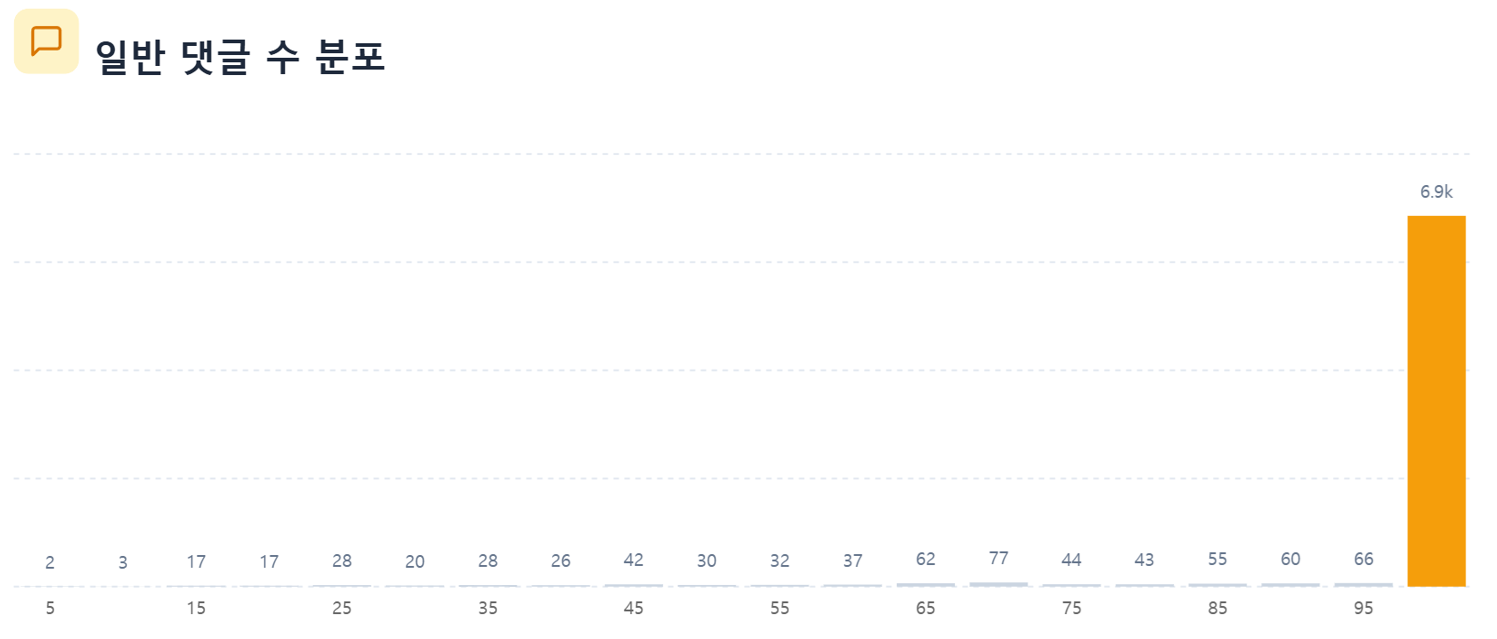
\includegraphics[width=\textwidth]{figures/raw_data_regular_comment.png}
         \caption{전체 일반 댓글 분포}
         \label{fig:overall_reg_sep}
     \end{subfigure}
     \hfill
     \begin{subfigure}[b]{0.48\textwidth}
         \centering
         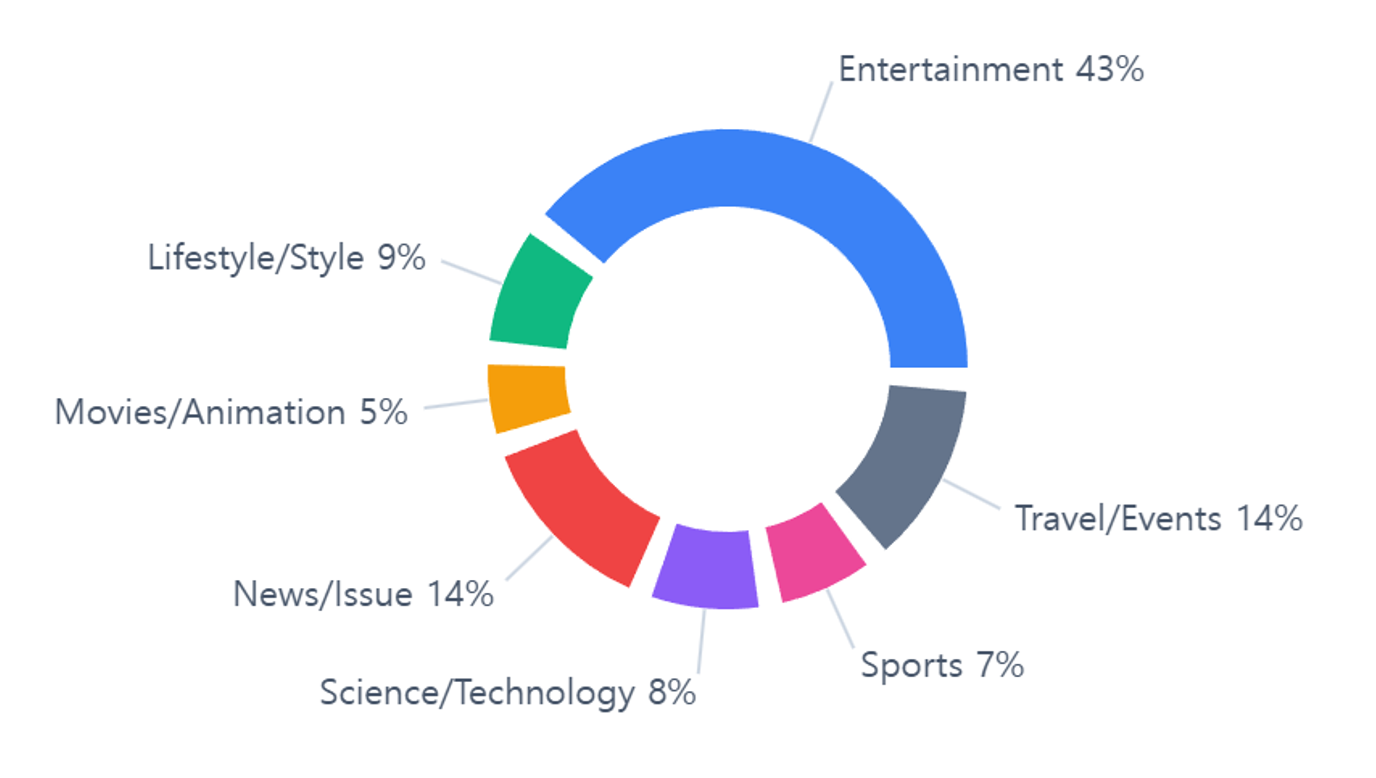
\includegraphics[width=\textwidth]{figures/raw_category_distribution.png}
         \caption{카테고리별 데이터 분포}
         \label{fig:cat_dist_sep}
     \end{subfigure}

     \vspace{1em}

     % 두 번째 행: 카테고리별 세부 비교 지표
     \begin{subfigure}[b]{0.48\textwidth}
         \centering
         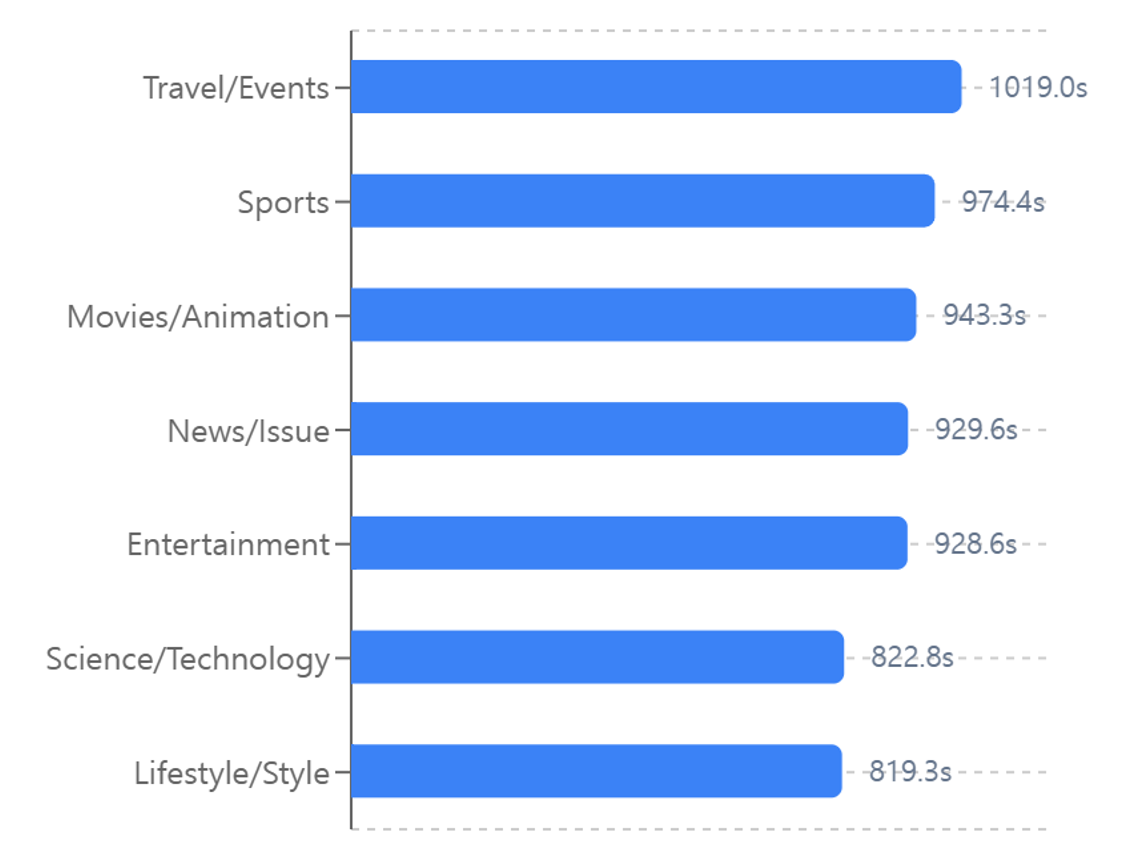
\includegraphics[width=\textwidth]{figures/raw_category_video_length.png}
         \caption{카테고리별 평균 영상 시간}
         \label{fig:cat_len_sep}
     \end{subfigure}
     \hfill
     \begin{subfigure}[b]{0.48\textwidth}
         \centering
         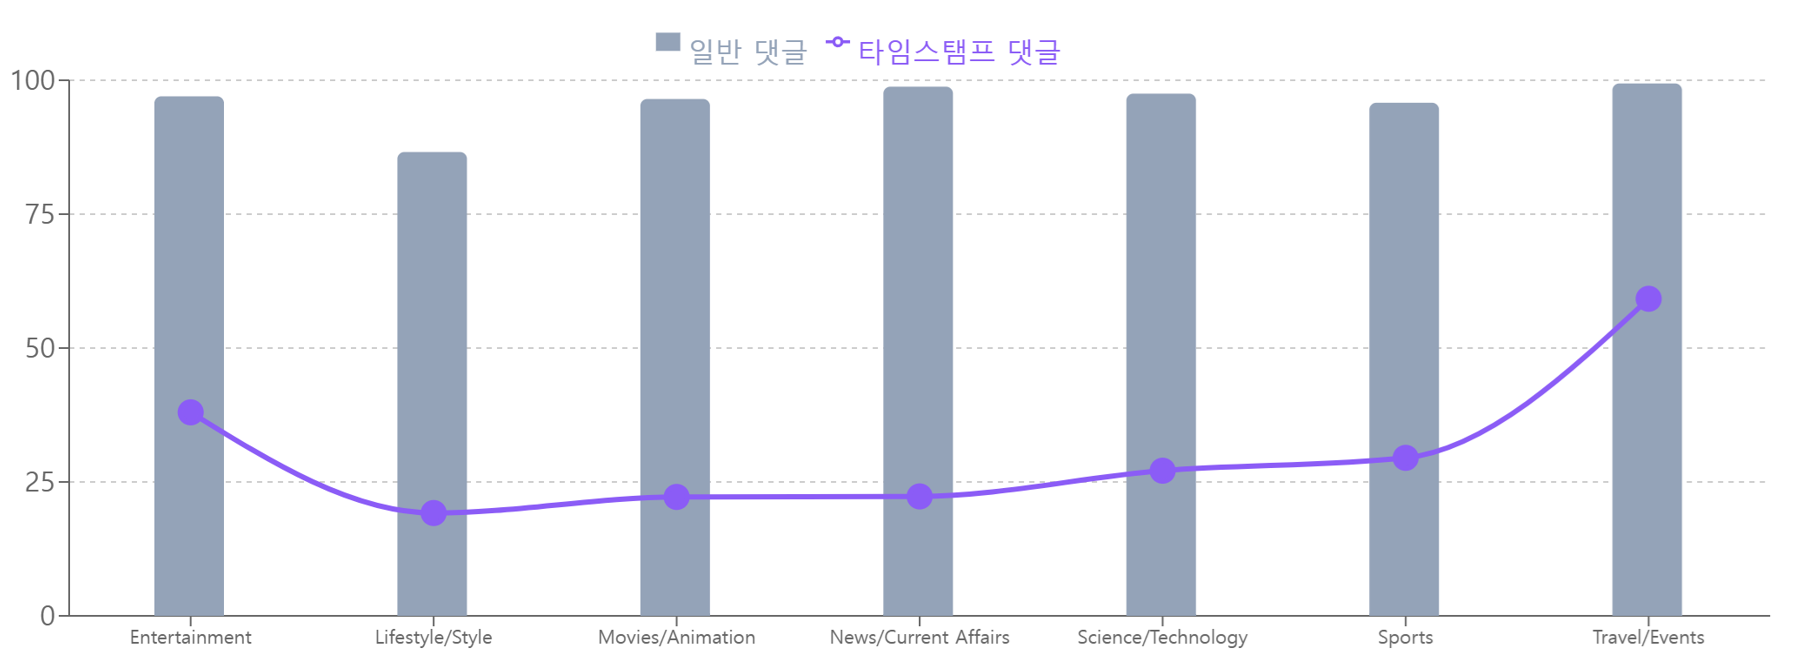
\includegraphics[width=\textwidth]{figures/raw_category_regular_timestamp_comment.png}
         \caption{카테고리별 댓글 비교}
         \label{fig:cat_comm_sep}
     \end{subfigure}
     
     \caption{원시데이터: 일반 댓글 분포 및 카테고리별 통계 지표}
     \label{fig:raw_dataset_stats}
\end{figure}


\end{document}

